\documentclass{beamer}
\usepackage[utf8]{inputenc}
\usepackage{graphicx}

\usetheme{Madrid}
\usecolortheme{default}

%------------------------------------------------------------
%This block of code defines the information to appear in the
%Title page
\title{Multi-armed bandit problem}

\subtitle{}

\author{}

\institute % (optional)
{}

\date % (optional)
{}


\setbeamertemplate{headline}{}

%------------------------------------------------------------


\begin{document}

%---------------------------------------------------------
    \begin{frame}
        \frametitle{Simulations for Stationary Multi-Armed Bandit Problem}
        Figure 1
        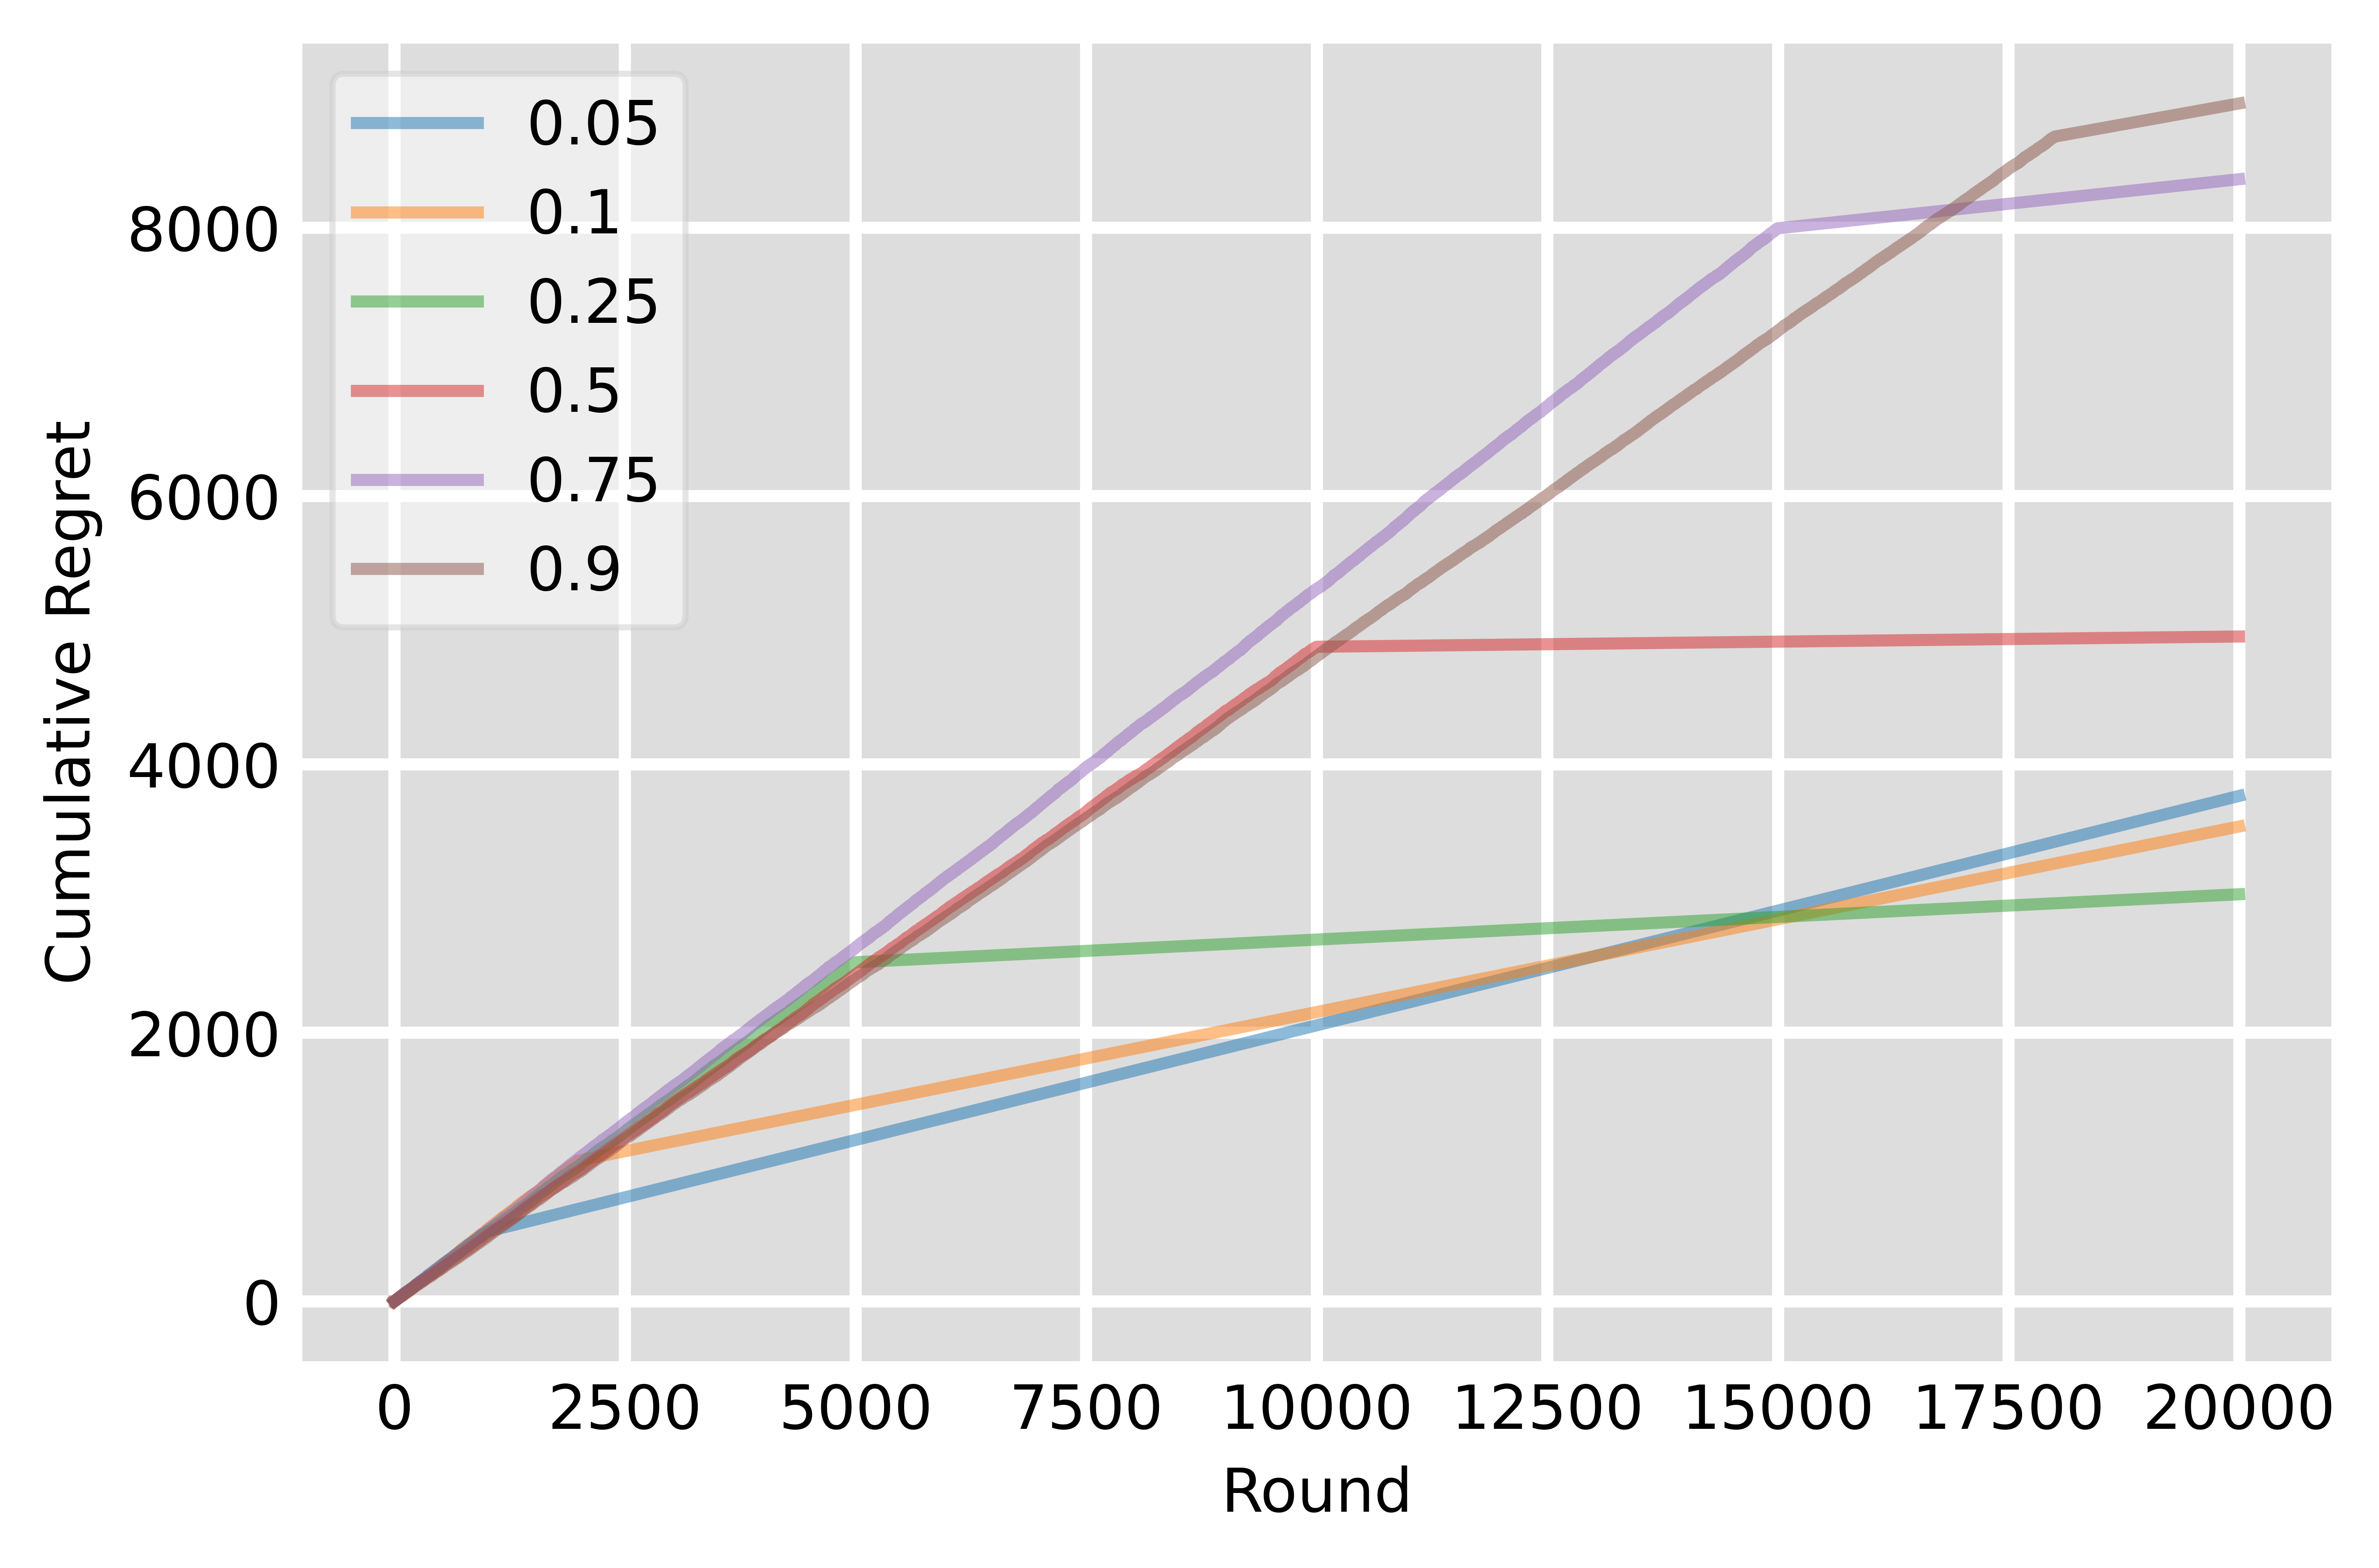
\includegraphics[width=0.9\textwidth]{../report/figures/epsilon_plot}
    \end{frame}

    \begin{frame}
        \frametitle{Simulations for Stationary Multi-Armed Bandit Problem}
        Figure 2
        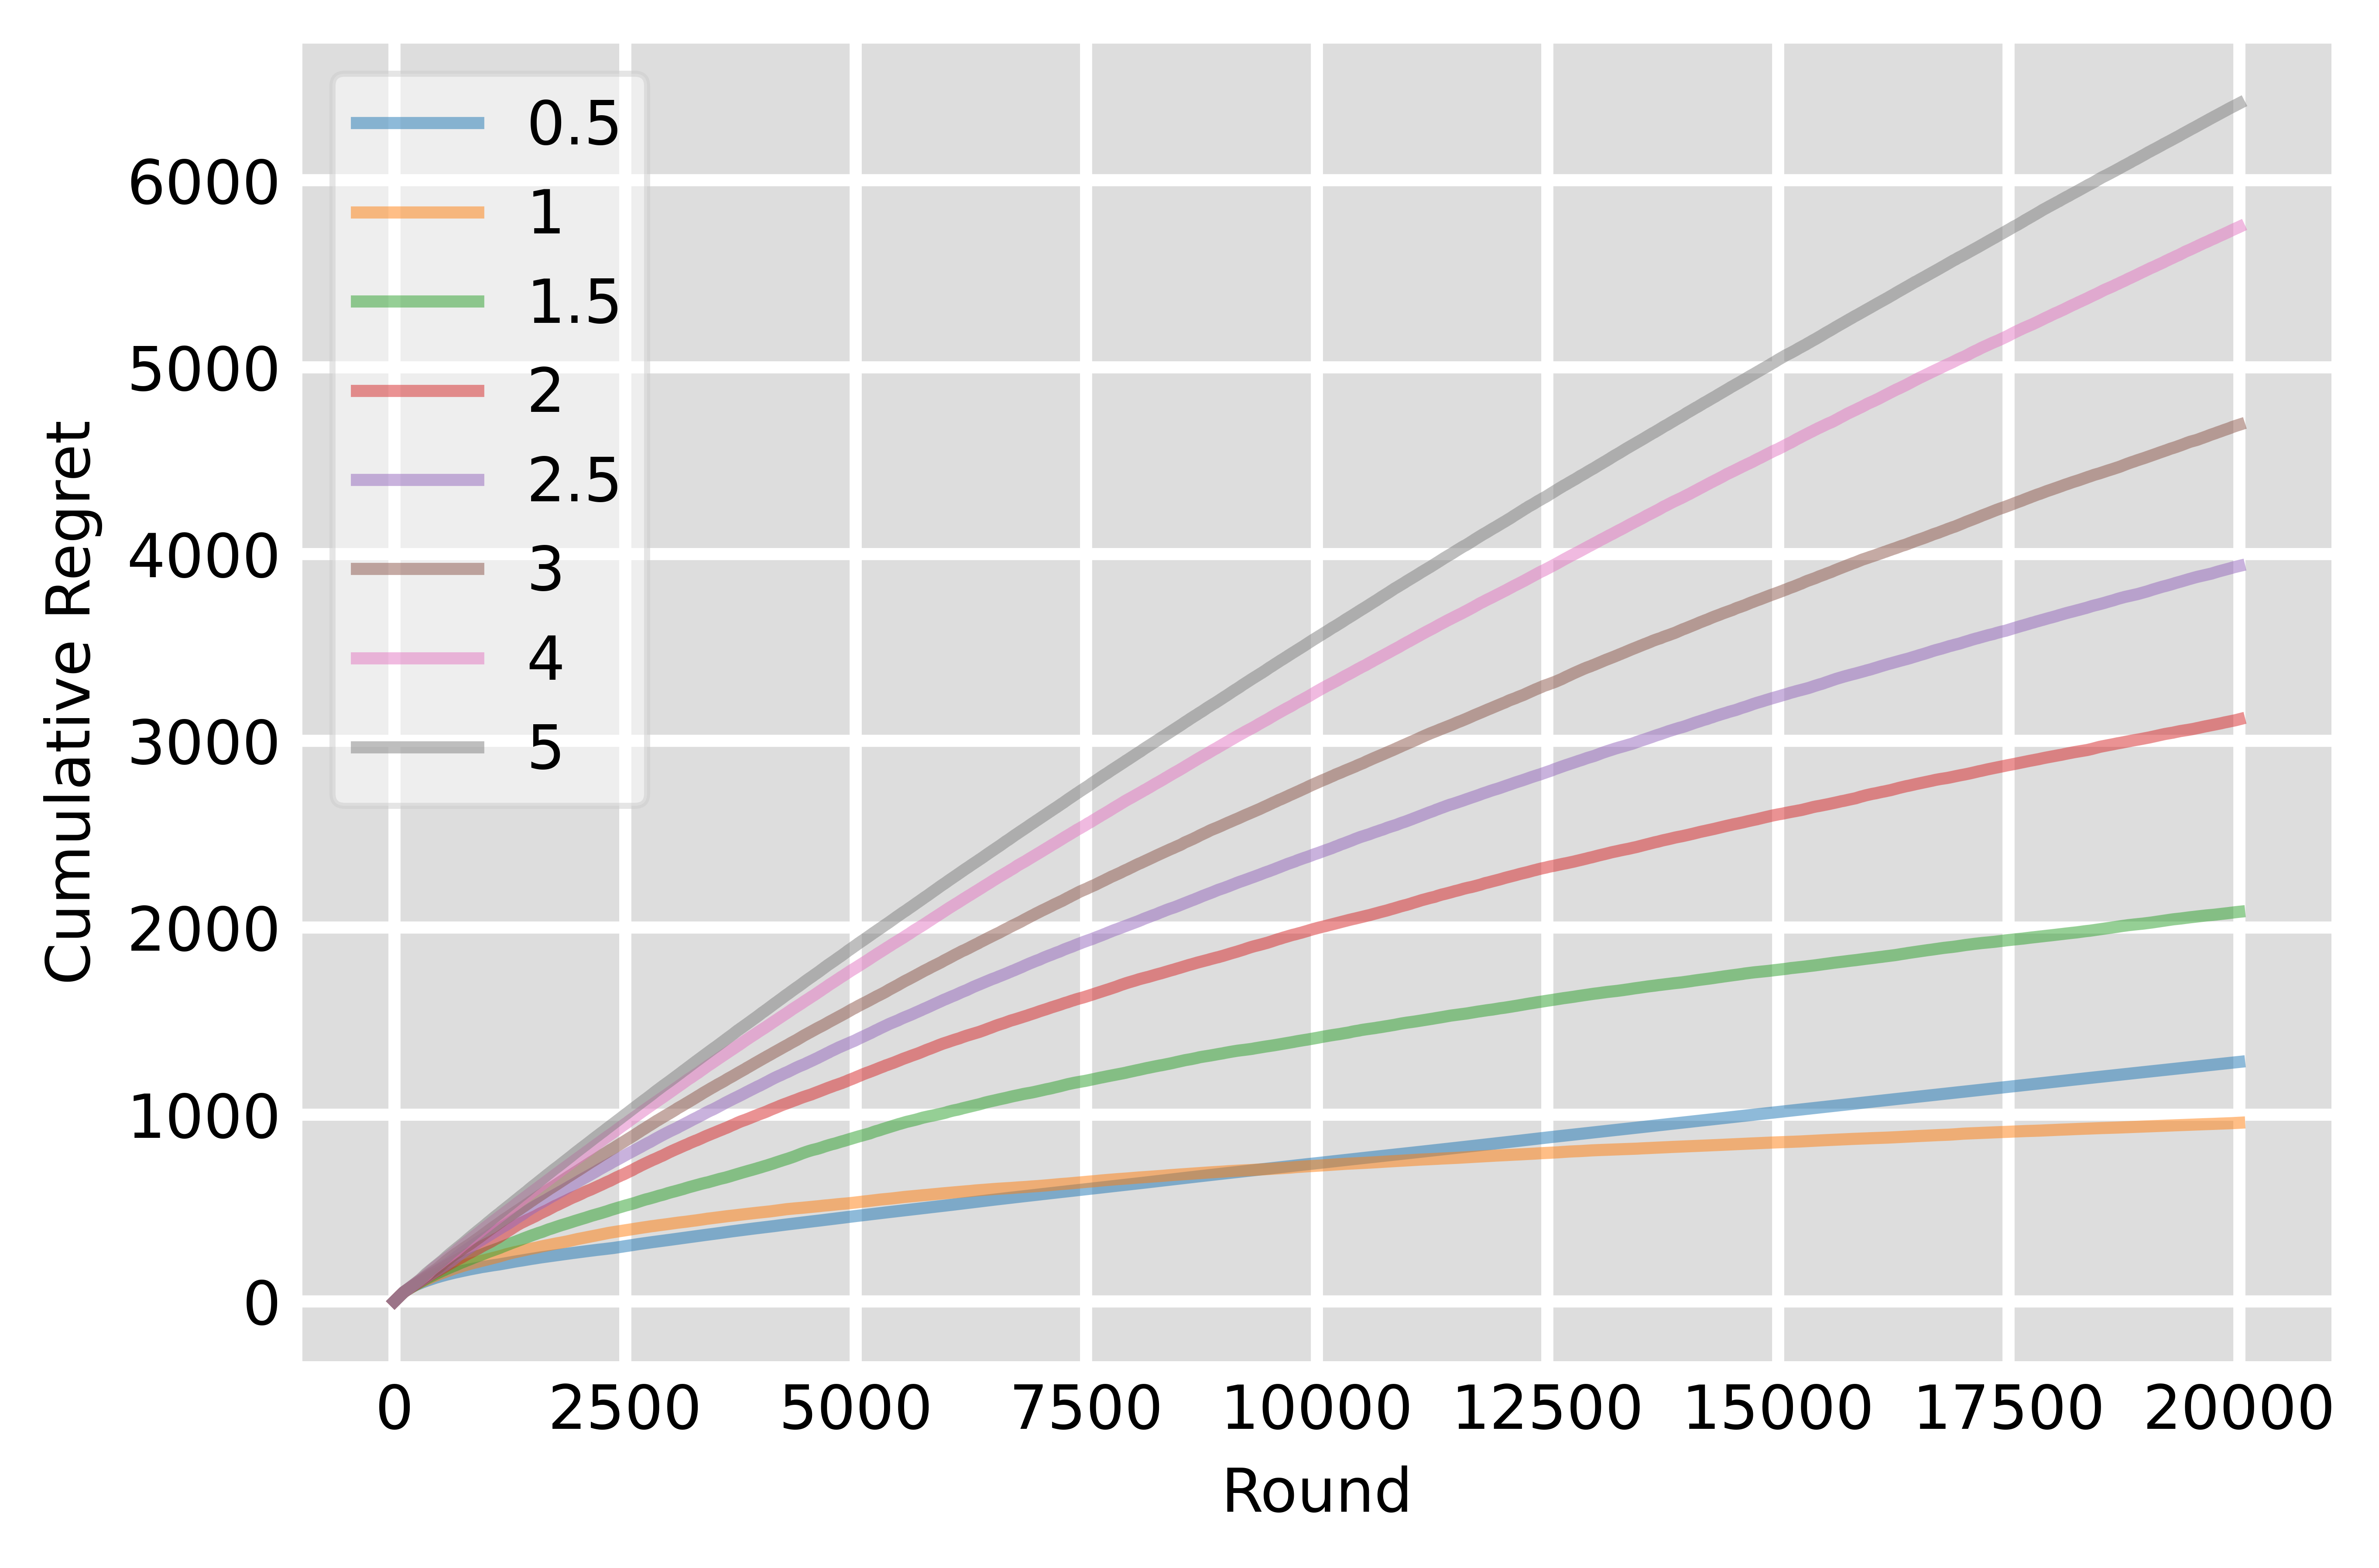
\includegraphics[width=0.9\textwidth]{../report/figures/ucb_plot}
    \end{frame}

    %---------------------------------------------------------

    %---------------------------------------------------------
    \begin{frame}
        \frametitle{Simulations for Stationary Multi-Armed Bandit Problem}
        Figure 3
        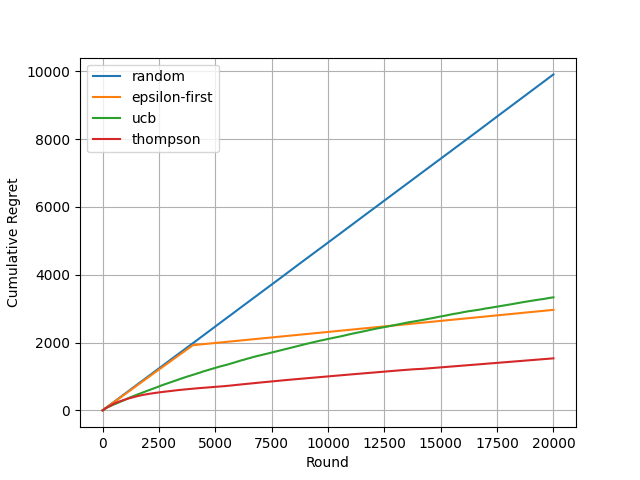
\includegraphics[width=0.85\textwidth]{../report/figures/100machines}
    \end{frame}
\end{document}